\documentclass[12pt, letterpaper]{article}
\usepackage{amsmath,amssymb,amsthm,amsopn,amscd}
\usepackage{mathtools}
\usepackage{latexsym}
\usepackage{graphicx,caption,subcaption}
\usepackage{multirow}
\usepackage[reftex]{theoremref}
\usepackage{hyperref}
\usepackage{verbatim}
\usepackage{color}
\usepackage{algorithm}      % pseudo-code
\usepackage{algpseudocode}  %
\usepackage{stmaryrd}       % double brackets
\usepackage{amstext}    % \text macro
\usepackage{array}      % \newcolumntype macro
\usepackage{tikz}       % for flow chart
\usetikzlibrary{cd}     % commutative diagram
\usetikzlibrary{shapes.geometric} % pentagon
\usetikzlibrary{calc}
\usetikzlibrary{patterns}
\usepackage{graphics, tkz-berge} % icosahedron
\usepackage{afterpage}
\usepackage[export]{adjustbox}
\usepackage{tensor}
\usepackage{braket}
\usepackage{etoolbox}
\usepackage{xparse}
\usepackage{titlesec}	% lv4 title
%\usepackage{subfigure}
\usepackage{mathrsfs}
\usepackage{pgfplots}
%   \usepackage{commath}    % for abs and norm

\usepackage{ytableau}
%\usepackage{geometry}		% change margin
\usepackage[margin=1.5in]{geometry} 		% change margin

%\setcounter{secnumdepth}{-2} % remove section numbering
\setcounter{section}{-1}

%\newcommand{\executeiffilenewer}[3]{%
%	\ifnum\pdfstrcmp{\pdffilemoddate{#1}}%
%	{\pdffilemoddate{#2}}>0%
%	{\immediate\write18{#3}}\fi%
%}
%\newcommand{\includesvg}[1]{%
%	\executeiffilenewer{#1.svg}{#1.pdf}%
%	{inkscape -z -D --file=#1.svg %
%		--export-pdf=#1.pdf --export-latex}%
%	\input{#1.pdf_tex}%
%}



\graphicspath{ {./} }

\makeatletter
\renewcommand\subparagraph{\@startsection{subparagraph}{5}{\parindent}%
	{3.25ex \@plus1ex \@minus .2ex}%
	{0.75ex plus 0.1ex}% space after heading
	{\normalfont\normalsize\bfseries}}
\makeatother

\newcommand\independent{\protect\mathpalette{\protect\independenT}{\perp}}
\def\independenT#1#2{\mathrel{\rlap{$#1#2$}\mkern2mu{#1#2}}}
\newcommand{\rp}{\mathbb{RP}}

\newcommand{\transpose}[1]{{{#1}^{\intercal}}}

%   Sets

\newcommand{\calS}{\mathcal{S}}
\newcommand{\calT}{\mathcal{T}}

\newcommand{\nat}{\mathbb{N}}
\newcommand{\inte}{\mathbb{Z}}
\newcommand{\rat}{\mathbb{Q}}
\newcommand{\re}{\mathbb{R}}
\newcommand{\renn}{\mathbb{R}_0^+}
\newcommand{\co}{\mathbb{C}}
\newcommand{\hil}{\mathbb{H}}
\newcommand{\field}{\mathbb{F}}
\newcommand{\ee}{\mathrm{e}}
\newcommand{\dd}{\mathrm{d}}
\newcommand{\GL}{\operatorname{GL}}
\newcommand{\SL}{\operatorname{SL}}
\newcommand{\PGL}{\operatorname{PGL}}
\newcommand{\PSL}{\operatorname{PSL}}
\newcommand{\MM}{\operatorname{M}}
\newcommand{\ZZ}{\operatorname{Z}}
\newcommand{\SZ}{\operatorname{SZ}}
\newcommand{\ob}{\operatorname{ob}}
\newcommand{\dom}{\operatorname{dom}}
\newcommand{\cod}{\operatorname{cod}}
\newcommand{\Hom}{\operatorname{Hom}}
\newcommand{\End}{\operatorname{End}}
\newcommand{\class}{\operatorname{class}}
\newcommand{\supp}{\operatorname{supp}}
\newcommand{\idt}{\operatorname{id}}
\newcommand{\sgn}{\operatorname{sgn}}
\newcommand{\Sym}{\operatorname{Sym}}
\newcommand{\Tr}{\operatorname{Tr}}
\newcommand{\Cl}{\operatorname{Cl}}
\newcommand{\Res}{\operatorname{Res}}
\newcommand{\Ind}{\operatorname{Ind}}

\newcommand{\ext}[1]{\bigwedge\!^{#1}}


\DeclarePairedDelimiter\ceil{\lceil}{\rceil}
\DeclarePairedDelimiter\floor{\lfloor}{\rfloor}


\newcommand{\id}{\indices}
%   \newcommand{\cp}{\mathbb{CP}}
%   \newcommand{\dS}{\mathbb{S}}
%   \newcommand{\dP}{\mathbb{P}}
%   \newcommand{\dE}{\mathbb{E}}
%   \newcommand{\dZ}{\mathbb{Z}}
\newcommand{\rmT}{\mathrm{T}}
\newcommand{\rmR}{\mathrm{R}}
\newcommand{\bfP}{\mathbf{P}}
\newcommand{\bfJ}{\mathbf{J}}
\newcommand{\bfK}{\mathbf{K}}
\newcommand{\bfR}{\mathbf{R}}
\newcommand{\idm}{\mathbf{I}}
\newcommand{\bfA}{\mathbf{A}}
\newcommand{\bfB}{\mathbf{B}}
\newcommand{\bfC}{\mathbf{C}}
\newcommand{\bfD}{\mathbf{D}}
\newcommand{\bfG}{\mathbf{G}}
\newcommand{\bfL}{\mathbf{L}}
\newcommand{\bfT}{\mathbf{T}}
\newcommand{\bfS}{\mathbf{S}}
\newcommand{\bfe}{\mathbf{e}}
%   \newcommand{\bm}{\boldsymbol{m}}
%   \newcommand{\bmu}{\boldsymbol{\mu}}
%   \newcommand{\bS}{\boldsymbol{\Sigma}}
%   \newcommand{\uvec}[1]{\mathrm{\mathbf{\hat{e}}}_#1}
%   \newcommand{\rmbf}[1]{\mathrm{\mathbf{#1}}}
%   \newcommand{\javg}{J_{\mathrm{avg^2}}}
%   \newcommand{\pgl}[1]{\mathbf{PGL}(#1,\mathbb{R})}
%   \newcommand{\Sl}[1]{\mathbf{SL}(#1,\mathbb{R})}
%   \newcommand{\gl}[1]{\mathbf{GL}(#1,\mathbb{R})}

\makeatletter
\newcommand\etc{etc\@ifnextchar.{}{.\@}}
\newcommand\ie{i.e\@ifnextchar.{}{.\@}}
\newcommand\eg{e.g\@ifnextchar.{}{.\@}}
\newcommand\Eq{Eq.\ }
\makeatother


\NewDocumentCommand\closure{sm}
{\IfBooleanTF{#1}{\overline{#2}}{\overline{#2}}}
\NewDocumentCommand\interior{sm}
{\IfBooleanTF{#1}{?}{\mathring{#2}}{}}

\newcommand{\red}[1]{{\color{red} #1}}
\newcommand{\blue}[1]{{\color{blue} #1}}		

\newcommand{\power}{\mathcal{P}}
\newcommand{\domain}{\mathcal{D}}

\newcommand{\opp}[1]{{#1}^{\mathrm{op}}}

\newcommand{\na}{\nabla}
\newcommand{\abs}[1]{\left\lvert #1 \right\rvert}
\newcommand{\card}[1]{\left\lvert #1 \right\rvert}
\newcommand{\norm}[1]{\left\lVert #1 \right\rVert}
\newcommand{\gaussian}{\mathcal{N}}
\newcommand{\define}{\coloneqq}
\newcommand{\tp}[1]{{#1}^T}
\newcommand{\hadj}[1]{{#1}^{\dagger}}
\newcommand{\conj}{\overline}
\renewcommand{\emptyset}{\varnothing}
\newcommand{\symdif}{\triangle}
%
%   \newcommand{\lst}[2]{\{#1_{1}, #1_{2}, \dots, #1_{#2}\}}
%   \newcommand{\lstf}[2]{\{#1{1}, #1{2}, \dots, #1{#2}\}}
%   % prt stands for parenthesis
%   \newcommand{\prt}[2]{(#1_{1}, #1_{2}, \dots, #1_{#2})}
%   \newcommand{\prtf}[2]{(#1{1}, #1{2}, \dots, #1{#2})}
%   % general list formatted, #1: fxn, #2: first one, #3: last one, #4: delimiter, #5: left, #6: right
%   \newcommand{\glstf}[6]{#5 #1{#2} #4 #1{\number\numexpr#2+1\relax} #4 \dots #4 #1{#3} #6}
%
% wc = wild card
\newcommand*{\wcthin}{{\mkern 2mu\cdot\mkern 2mu}}
\newcommand*{\wc}{{}\cdot{}}    %   This one is wider
%
% Operators
% ec = equivalence class
\newcommand{\ec}[1]{\left[{#1}\right]}
% generating subgroup
\newcommand{\gensub}[1]{\left\langle{#1}\right\rangle}
%
%   automatic math mode in tabular
\newcolumntype{L}{>{$}l<{$}}
\newcolumntype{C}{>{$}c<{$}}
\newcolumntype{R}{>{$}r<{$}}

\newenvironment{centabular}{\center\tabular}{\endtabular\endcenter}
\newenvironment{centikzpic}{\center\tikzpicture}{\endtikzpicture\endcenter}
\newenvironment{centikzcd}{\center\tikzcd}{\endtikzcd\endcenter}
\newenvironment{eqlong}{\equation\aligned}{\endaligned\endequation}


\DeclareMathOperator*{\argmin}{arg\,min}
\DeclareMathOperator*{\argmax}{arg\,max}
\DeclareMathOperator{\Var}{Var}
\DeclareMathOperator{\Cov}{Cov}
\DeclareMathOperator{\rank}{rank}
\DeclareMathOperator{\spn}{span}
\DeclareMathOperator{\diag}{diag}
\DeclareMathOperator{\tr}{tr}

\newtheorem*{prop*}{Proposition}
\newtheorem{prop}{Proposition}[section]
\newtheorem*{lem*}{Lemma}
\newtheorem{lem}[prop]{Lemma}
\newtheorem{cor}[prop]{Corollary}
\newtheorem{thm}[prop]{Theorem}
\newtheorem*{thm*}{Theorem}
\newtheorem{conjec}[prop]{Conjecture}


%\titleformat{\paragraph}
%{\normalfont\normalsize\bfseries}{\theparagraph}{1em}{}
%\titlespacing*{\paragraph}
%{0pt}{3.25ex plus 1ex minus .2ex}{1.5ex plus .2ex}

%\makeatletter
%\renewcommand\paragraph{\@startsection{paragraph}{4}{\z@}%
%	{3.25ex \@plus1ex \@minus.2ex}%
%	{-1em}%
%	{\normalfont\normalsize\bfseries}}
%\renewcommand\subparagraph{\@startsection{subparagraph}{5}{\parindent}%
%	{3.25ex \@plus1ex \@minus .2ex}%
%	{-1em}%
%	{\normalfont\normalsize\bfseries}}
%%\def\toclevel@subsubsubsection{4}
%\def\toclevel@paragraph{4}
%\def\toclevel@paragraph{5}
%\def\toclevel@definition{6}
%%\def\l@subsubsubsection{\@dottedtocline{4}{7em}{4em}}
%%\def\l@paragraph{\@dottedtocline{4}{10em}{5em}}
%%\def\l@subparagraph{\@dottedtocline{5}{14em}{6em}}
%%\def\l@definition{\@dottedtocline{6}{15em}{7em}}
%\def\l@paragraph{\@dottedtocline{4}{6em}{4em}}
%\def\l@subparagraph{\@dottedtocline{5}{8em}{5em}}
%\def\l@definition{\@dottedtocline{6}{8.5em}{0em}}
%\makeatother
%
%\setcounter{secnumdepth}{6}
%\setcounter{tocdepth}{6}

%https://tex.stackexchange.com/questions/280313/how-to-put-the-list-of-definitions-at-contents-page
%https://tex.stackexchange.com/questions/51691/creating-list-of-for-newtheoremstyle
%\usepackage{amsthm}
%\newtheoremstyle{mystyle}
%{\topsep}{\topsep}{}{}{\bfseries}{:}{\newline}
%{\thmname{#1}\thmnumber{ #2}\thmnote{ (#3)}%
%	\ifstrempty{#3}%
%	{\addcontentsline{def}{subsection}{#1~\thedef}}%
%	{\addcontentsline{def}{subsection}{#1~\thedef~(#3)}}}
%
%\theoremstyle{mystyle}
%\newtheorem*{def*}{Definition}
\theoremstyle{definition}
\newtheorem*{defaux}{Definition}

%https://tex.stackexchange.com/questions/60872/ams-theorems-in-table-of-contents
\NewDocumentEnvironment{def*}{o}
{\IfNoValueTF{#1}
	{\defaux\addcontentsline{toc}{definition}{\protect\numberline{}Definition}}
	{\defaux[#1]\addcontentsline{toc}{definition}{\protect\numberline{}Definition (#1)}}%
	\ignorespaces}
{\label{#1}}
{\enddefaux}

%\makeatletter
%\newcommand\definitionname{Definition}
%\newcommand\listdefinitionname{List of Definitions}
%\newcommand\listofdefinitions{%
%	\section*{\listdefinitionname}\@starttoc{def}}
%\makeatother

\theoremstyle{remark}
\newtheorem*{rem*}{Remark}
\newtheorem*{ack*}{Acknowledgements}

\theoremstyle{definition}
\newtheorem{exe}{Exercise}[section]
\newtheorem{exe*}[exe]{Exercise*}
\newtheorem{exam}[exe]{Example in Book}
\newtheorem{eq}[exe]{Equation in Book}
\newtheorem{ddef}[exe]{Definition in Book}
\theoremstyle{plain}
\newtheorem{pprop}[exe]{Proposition in Book}
\newtheorem{ccor}[exe]{Corollary in Book}
\newtheorem{llem}[exe]{Lemma in Book}
\newtheorem{tthm}[exe]{Theorem in Book}
\captionsetup{width=0.9\textwidth}


%%  \usetikzlibrary{shadows}% for shadow
%%  \tikzstyle{event} = [color=black!40,text=white,text centered,circular drop shadow,font=\large\bfseries,text height=4em,text width=4em]
%   \tikzstyle{event} = [draw, circle]
%   \tikzstyle{arrow} = [thick,->,>=stealth]
%%  \usetikzlibrary{arrows}
%%  \tikzstyle{arrow} = [draw, -latex', thick]
%
%   %only for this doc
%   \newcommand{\llb}{\llbracket}
%   \newcommand{\rrb}{\rrbracket}

%opening
\title{Reading Notes for \\ \large \textit{Category Theory} \\ by Steve Awodey}
\author{Zhi Wang}

\numberwithin{equation}{section}


\begin{document}
	
	\cleardoublepage
	\ytableausetup{centertableaux}
	
	\maketitle
	
	
	% https://tex.stackexchange.com/questions/154464/page-numbering-in-table-of-contents
	
	% Let's change \thepage so it prints one less than
	% the real page number; \pagenumbering{arabic}
	% will redefine it to the right meaning afterwards.
	\renewcommand\thepage{\romannumeral\numexpr\value{page}\relax}
	
	\tableofcontents
	
	%	\listofdefinitions
	
	\cleardoublepage
	\pagenumbering{arabic}
	
	
	\section{Notes and Definitions}
	\subsection{Notes}
	
	\section{Categories}
	\subsection{Introduction}
	\subsection{Functions of sets}
	\subsection{Definition of a category}
	\subsection{Examples of categories}
	\paragraph{1}
	\subparagraph{Functions with fibers of at most 2 elements}
	Assume
	\[\forall A,B\in \bfC\, \forall (f\colon A\to B )\,\Big[
	 \forall b\in B\big(\card{f^{-1}(b)}\le 2\big) \iff f\in \Hom_\bfC(A,B)  \Big].  \]
	
	Given that
	\[ \forall B\in\bfC\forall b\in B \Big[\card{1_B^{-1}(b)}=1\le 2\Big] , \]
	we know 
	\[ \forall B\in\bfC \Big[ 1_B\in\Hom_\bfC(B,B)\Big ]. \]
	
	Given $\forall A,B,C\in \bfC,\forall (f\colon A\to B) \,\forall (g\colon B\to C)$
	\[  \forall b\in B\Big(\card{f^{-1}(b)}\le 2\Big) \land  \forall c\in C\Big(\card{g^{-1}(b)}\le 2\Big) 
	\implies \forall c\in C \Big(\card{(g\circ f)^{-1}(c)}\le 4\Big)
	 \]
	which means that the composite $g\circ f$ does not necessarily exist in $\Hom_\bfC(A,B)$.
	
	Therefore, this is \textbf{not} a category.
	
	%https://tex.stackexchange.com/questions/402265/draw-concentric-boxes-around-elements-of-matrix-tikz
	%https://tex.stackexchange.com/questions/377608/animated-tikz-matrix-inside-a-flowchart-node
	%https://tex.stackexchange.com/questions/408497/box-around-tikz-cd-diagram-without-ampersand-replacement
	%https://tex.stackexchange.com/questions/409076/tikz-matrix-with-dotted-node-borders-but-not-on-the-first-row
	%https://dudebout.com/files/pdfs/matrix.skeleton-manual.pdf
	
	\begin{centikzcd}[remember picture,
		%row 1/.style={
		%	nodes={draw=gray, solid, fill=gray!50!white,font=\bfseries, text centered}}
		%%%%
		%boxedcd={inner sep=1pt}
		%%%%
		every matrix/.append style={column sep=tiny, name=fibertwo
			%, rows={draw=red}
		}]
		a_1\ar[rd,"f"]&&a_2\ar[ld,"f"']&&a_3\ar[rd,"f"]&&a_4\ar[ld,"f"']\\
		&b_1\ar[rrd,"g"]&&&&b_2\ar[lld,"g"']&\\
		&&&c&&&
	\end{centikzcd}
	\begin{tikzpicture}[remember picture, overlay]
		\def\mid{40}
		\draw[blue,rounded corners] ([xshift=0pt]fibertwo.south west) rectangle ([xshift=15pt, yshift=15pt]fibertwo.south east)
		node [black, below left] {$C$};
		\draw[blue,rounded corners] ([xshift=0pt,yshift=37.5 pt]fibertwo.south west) rectangle
		([xshift=15pt, yshift=52.5 pt]fibertwo.south east)
		node [black, below left] {$B$};
		\draw[blue,rounded corners] ([xshift=0pt]fibertwo.north west) rectangle ([xshift=15pt, yshift=-15pt]fibertwo.north east)
		node [black, above left] {$A$};
		% -- ([yshift=0pt]fibertwo.north east) -- ([yshift=0pt]fibertwo.north west) -- cycle; 
	\end{tikzpicture}

	\subparagraph{Functions with finite fiber}
	Assume
	\[\forall A,B\in \bfC\, \forall (f\colon A\to B )\,\Big[
	\forall b\in B\big(\card{f^{-1}(b)} \in\nat \big) \iff f\in \Hom_\bfC(A,B)  \Big].  \]
	
	Given that
	\[ \forall B\in\bfC\forall b\in B \Big[\card{1_B^{-1}(b)}=1\in \nat\Big] , \]
	we know 
	\[ \forall B\in\bfC \Big[ 1_B\in\Hom_\bfC(B,B)\Big ]. \]
	
	Given $\forall A,B,C\in \bfC,\forall (f\colon A\to B) \,\forall (g\colon B\to C)$
	\[  \forall b\in B\Big(\card{f^{-1}(b)}\in\nat\Big) \land  \forall c\in C\Big(\card{g^{-1}(b)}\in\nat\Big) 
	\iff \forall c\in C \Big(\card{(g\circ f)^{-1}(c)}\in\nat\Big)
	\]
	since the multiplication of finite numbers are finite, and converse is true.
	This means that the composite $g\circ f$ must exist in $\Hom_\bfC(A,B)$.
	
	Therefore, this \textbf{is} a category.
	
	\subparagraph{Functions with infinite fiber}
	Since identity map has finite fiber, this is \textbf{not} a category.
	
	\paragraph{2}
	\begin{itemize}
		\red{
		\item graphs and graph homomorphisms
		\item the real numbers $R$ and continuous functions $R \to R$,
		\item the natural numbers $N$ and all recursive functions $N \to N$, or as in
		the example of continuous functions, one can take partial recursive
		functions defined on subsets $U \subseteq N$}
	\end{itemize}
	%\setcounter{section}{10}
	\paragraph{11}
	
	\red{Category of data types and programs}
	
	Let's define a procedure as
	\texttt{
		Int f(Int a, Int b) {
			return a * b;
		}
	}

	We have built a morphism/arrow
	
	\[\texttt{f}\colon \texttt{Int}\times \texttt{Int}\to \texttt{Int}.\]
	
	\begin{figure}[H]
		\centering
		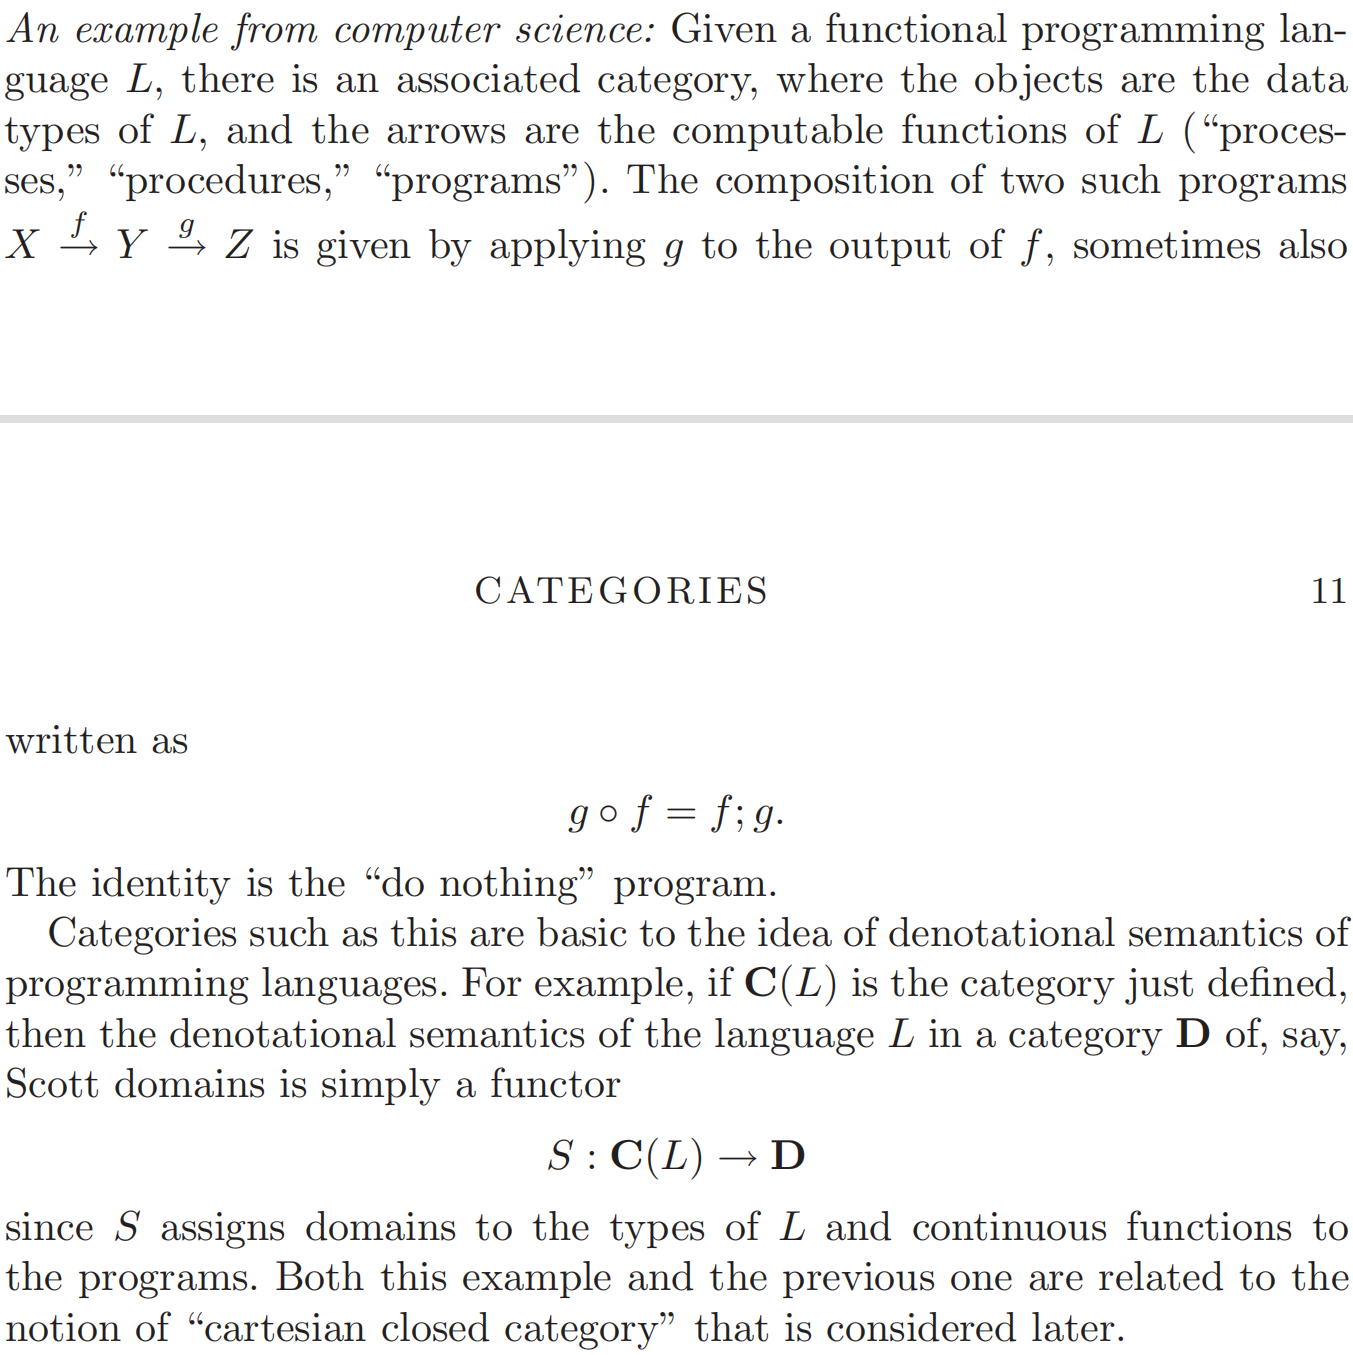
\includegraphics[width=0.7\linewidth]{1.4_11}
		\caption{}
		\label{fig:1}
	\end{figure}
	
	\subsection{Isomorphisms}
	\paragraph{Definition 1.3}
	while there are ``bijective homomorphisms''
	between non-isomorphic posets.
	
	\blue{The inverse must also be homomorphism?}
	
	\paragraph{Theorem 1.6}
	
	\red{Every category (big or small) is isomorphic to a concrete (small) category.
	So what make those big?}

	\[\red{f,h\in \bar{C}}, \blue{g\circ f,g\circ h\in \bar{D}}.\]
	\begin{centikzcd}[
			remember picture,
			every matrix/.append style={name=arrows}
		]
		X\ar[d,red,"f"']\ar[rd,blue,"g\circ f"]&\\
		C\ar[r,purple,"g"]&D&&\red{\bar{C}}\ar[r,purple,"\bar{g}"] & \blue{\bar{D}} \\
		Y\ar[u,red,"h"]\ar[ru,blue,"g\circ h"']&
	\end{centikzcd}
	%\begin{tikzpicture}[remember picture, overlay]
	%	\def\mid{40}
	%	\draw[red,rounded corners] ([xshift=0pt]arrows.south west) rectangle ([xshift=17.5pt, yshift=15pt]arrows.north west)
	%	node [below left] {$\bar{C}$};
	%\end{tikzpicture}

	
	\paragraph{Remark 1.7}
	\subparagraph{}
	
	\red{What does this mean}
	\begin{figure}[H]
		\centering
		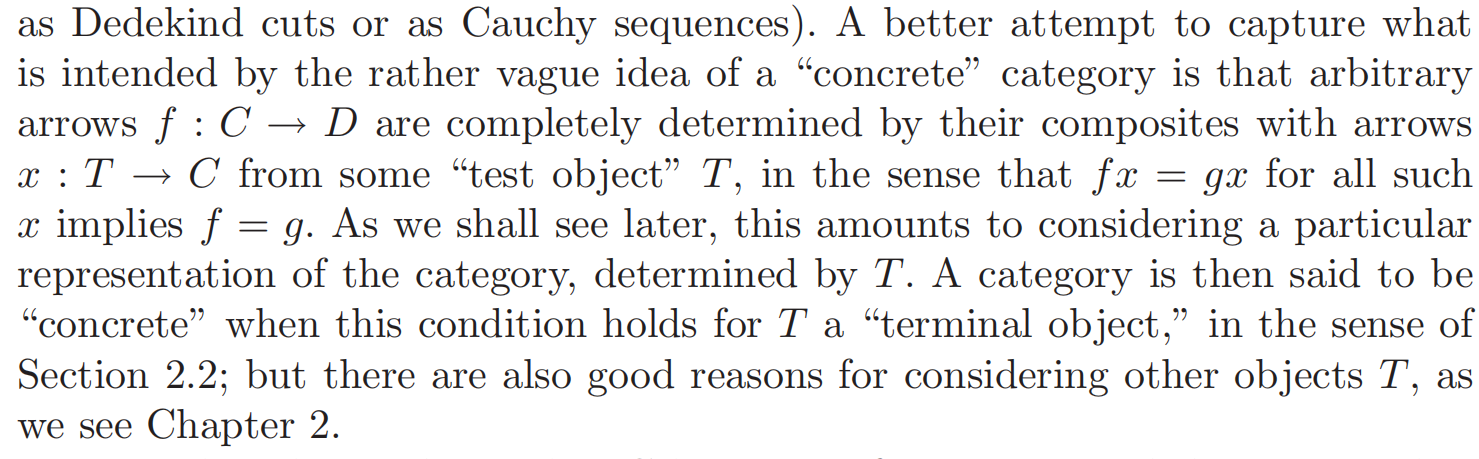
\includegraphics[width=0.7\linewidth]{1.5_1.7}
		\caption{}
		\label{fig:2}
	\end{figure}
	
	\subparagraph{}
	\blue{If the arrows in the category is too large to form a set, then it might not be isomorphic to a small category?}
	
	\subsection{Constructions on categories}
	\paragraph{3 The arrow category}
	
	\begin{centikzcd}
		A\ar[r,"g_1"]\ar[d,"f"]&A'\ar[r,"h_1"]\ar[d,"f'"]&A''\ar[d,"f''"]\\
		B\ar[r,"g_2"]&B'\ar[r,"h_2"]&B''
	\end{centikzcd}
	
\end{document}